\subsubsection{Prototyp}
\label{sec:Prototyp}

Nach der Bereitstellung des Ticketsystems und des Versionierungstools kann mit
der Implementierung der Software begonnen werden. Für die Auftraggeber des
Projektes war es dabei besonders wichtig, dass zunächst ein Prototyp der
späteren Software entwickelt wird. Dieser Prototyp soll zur Entwicklung einer
gemeinsamen Vorstellung vom Projekt zwischen Auftraggeber und Projektteam
dienen. Der Prototyp soll hierbei nur die Rundumansicht in einem
360-Grad-Foto und die Möglichkeit, zu einem weiteren Panoramafoto zu navigieren,
enthalten.

Da der Prototyp nur einen statischen Einblick in die späteren Benutzeransicht
gewähren sollte und keine Inhalte dynamisch aus der Datenbank geladen werden
müssen, wurde hierfür ein HTML-Dokument geschrieben, das die Google Street View
API einbindet und über Javascript dessen Funktionalität implementiert. Das
erstellte HTML-Dokument ist in \listing{HTML Prototyp} dargestellt:

\lstinputlisting[language=HTML,caption={HTML Prototyp},label={lst:HTML Prototyp}]{Listings/HTML_Prototyp.html}

Das dargestellte HTML-Dokument bindet in Zeile 5 die angesprochene Google
Street View API ein, in der die Funktionen zur Darstellung des 360-Grad-Fotos
definiert sind. Zusätzlich wird in Zeile 6 eine Javascript-Datei eingebunden,
in der die Funktionen der Google Street View API auferufen werden. Im
Body-Bereich des HTML-Dokumentes ist dafür ein Element definiert das als Fläche
zur Darstellung der Panoramas genutzt wird. Die eingebundene Javascript-Datei
aus Zeile 6 ist aus Gründen der Übersichtlichkeit
im Anhang~\ref{sec:AnhangJavascriptPrototyp} dargestellt. Dessen Funktionalität
wird an dieser Stelle kurz erläutert.

Sobald der Internetbrowser des Benutzers das HTML-Dokument vollständig geladen
hat, wird eine Methode aufgerufen, die die benötigten Parameter zur Erstellung
des Panoramas bereitstellt\footnote{Vergleiche Zeile 3 im Anhang
~\ref{sec:AnhangJavascriptPrototyp}}. Hier werden Zoomstufe, Ausrichtung und
weitere Parameter festgelegt. Anschließend wird ein Panorama-Objekt mithilfe
der Google Street View API erstellt und an das oben beschriebene HTML-Element
im Body-Bereich gebunden\footnote{Vergleiche Zeile 16-18 im Anhang
~\ref{sec:AnhangJavascriptPrototyp}}. Über einen weiteren Aufruf einer
API-Funktion können an das Panorama sogenannte "`Links"' gehängt werden. Diese
Links stellen später für den Benutzer die Pfeile dar über die zu anderen
Panoramas navigiert werden kann. Im Prototyp wird nur der Verweis auf ein
anderes Panorama gebraucht, welches über die Funktion
"`createCustomLinks"'\footnote{Vergleiche Zeile 45ff. im Anhang
~\ref{sec:AnhangJavascriptPrototyp}} als Link angehängt wird.

Ein Bildschirmfoto des Prototypen der mit den beschriebenen HTML- und
Javascript-Dateien erstellt wurde ist in \abbildung{PrototypScreenshot} zu
sehen.

\begin{figure}[htb]
\centering
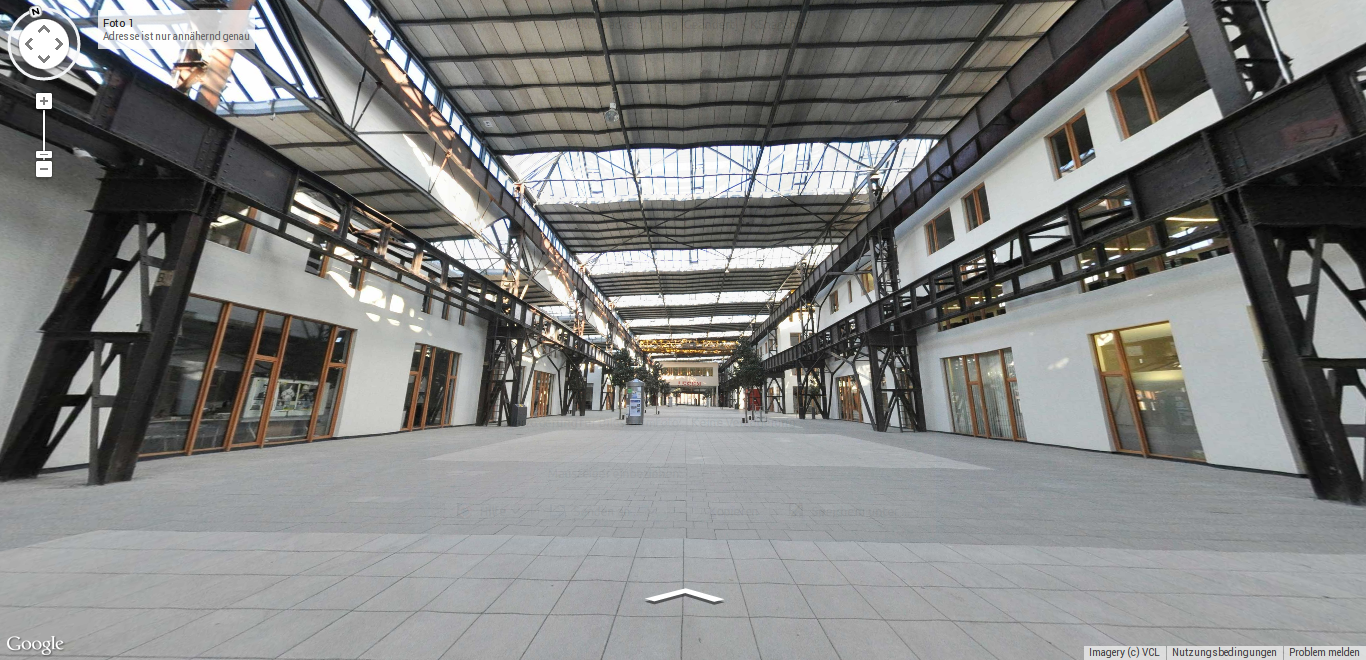
\includegraphics[width=1.0\textwidth]{PrototypScreenshot.png}
\caption[Protoyp Bildschirmfoto]{Bildschirmfoto des Prototypen}
\label{fig:PrototypScreenshot}
\end{figure}